% Options for packages loaded elsewhere
\PassOptionsToPackage{unicode}{hyperref}
\PassOptionsToPackage{hyphens}{url}
%
\documentclass[
  12pt,
  ignorenonframetext,
  aspectratio=169,
]{beamer}
\usepackage{pgfpages}
\setbeamertemplate{caption}[numbered]
\setbeamertemplate{caption label separator}{: }
\setbeamercolor{caption name}{fg=normal text.fg}
\beamertemplatenavigationsymbolsempty
% Prevent slide breaks in the middle of a paragraph
\widowpenalties 1 10000
\raggedbottom
\setbeamertemplate{part page}{
  \centering
  \begin{beamercolorbox}[sep=16pt,center]{part title}
    \usebeamerfont{part title}\insertpart\par
  \end{beamercolorbox}
}
\setbeamertemplate{section page}{
  \centering
  \begin{beamercolorbox}[sep=12pt,center]{part title}
    \usebeamerfont{section title}\insertsection\par
  \end{beamercolorbox}
}
\setbeamertemplate{subsection page}{
  \centering
  \begin{beamercolorbox}[sep=8pt,center]{part title}
    \usebeamerfont{subsection title}\insertsubsection\par
  \end{beamercolorbox}
}
\AtBeginPart{
  \frame{\partpage}
}
\AtBeginSection{
  \ifbibliography
  \else
    \frame{\sectionpage}
  \fi
}
\AtBeginSubsection{
  \frame{\subsectionpage}
}
\usepackage{lmodern}
\usepackage{amssymb,amsmath}
\usepackage{ifxetex,ifluatex}
\ifnum 0\ifxetex 1\fi\ifluatex 1\fi=0 % if pdftex
  \usepackage[T1]{fontenc}
  \usepackage[utf8]{inputenc}
  \usepackage{textcomp} % provide euro and other symbols
\else % if luatex or xetex
  \ifxetex
    \usepackage{mathspec}
  \else
    \usepackage{unicode-math}
  \fi
  \defaultfontfeatures{Scale=MatchLowercase}
  \defaultfontfeatures[\rmfamily]{Ligatures=TeX,Scale=1}
\fi
\usetheme[]{Dresden}
\usecolortheme{dolphin}
\usefonttheme{structurebold}
% Use upquote if available, for straight quotes in verbatim environments
\IfFileExists{upquote.sty}{\usepackage{upquote}}{}
\IfFileExists{microtype.sty}{% use microtype if available
  \usepackage[]{microtype}
  \UseMicrotypeSet[protrusion]{basicmath} % disable protrusion for tt fonts
}{}
\makeatletter
\@ifundefined{KOMAClassName}{% if non-KOMA class
  \IfFileExists{parskip.sty}{%
    \usepackage{parskip}
  }{% else
    \setlength{\parindent}{0pt}
    \setlength{\parskip}{6pt plus 2pt minus 1pt}}
}{% if KOMA class
  \KOMAoptions{parskip=half}}
\makeatother
\usepackage{xcolor}
\IfFileExists{xurl.sty}{\usepackage{xurl}}{} % add URL line breaks if available
\IfFileExists{bookmark.sty}{\usepackage{bookmark}}{\usepackage{hyperref}}
\hypersetup{
  pdftitle={Statistical Thinking in Biology Research},
  pdfauthor={Terry Neeman},
  hidelinks,
  pdfcreator={LaTeX via pandoc}}
\urlstyle{same} % disable monospaced font for URLs
\newif\ifbibliography
\usepackage{graphicx,grffile}
\makeatletter
\def\maxwidth{\ifdim\Gin@nat@width>\linewidth\linewidth\else\Gin@nat@width\fi}
\def\maxheight{\ifdim\Gin@nat@height>\textheight\textheight\else\Gin@nat@height\fi}
\makeatother
% Scale images if necessary, so that they will not overflow the page
% margins by default, and it is still possible to overwrite the defaults
% using explicit options in \includegraphics[width, height, ...]{}
\setkeys{Gin}{width=\maxwidth,height=\maxheight,keepaspectratio}
% Set default figure placement to htbp
\makeatletter
\def\fps@figure{htbp}
\makeatother
\setlength{\emergencystretch}{3em} % prevent overfull lines
\providecommand{\tightlist}{%
  \setlength{\itemsep}{0pt}\setlength{\parskip}{0pt}}
\setcounter{secnumdepth}{-\maxdimen} % remove section numbering
\usepackage{fancyvrb}

\title{Statistical Thinking in Biology Research}
\subtitle{Statistical Models}
\author{Terry Neeman}
\date{30th July 2020}
\institute{Australian National University}

\begin{document}
\frame{\titlepage}

\begin{frame}{A few key ideas}
\protect\hypertarget{a-few-key-ideas}{}

\begin{itemize}
\tightlist
\item
  Data are a measured response under a set of conditions.
\item
  The measured response is a mixture of ``signal'' and ``noise''
\item
  Noise: measurement error, biological, environmental variation
\item
  Statistical models turn data into information.
\end{itemize}

\begin{block}{The goal of statistical modelling is to partition data
into ``signal'' and ``noise'' or variation.}

\end{block}

\begin{block}{``Signal'' is average treatment effect or an association
between sets of variables and outcome.}

\end{block}

\end{frame}

\begin{frame}{What is a Statistical Model?}
\protect\hypertarget{what-is-a-statistical-model}{}

\begin{itemize}
\tightlist
\item
  An informative summary of data
\item
  A description of a data generating process
\item
  A mathematical model that includes measures of uncertainty
\end{itemize}

One can fit a model to \textbf{explain} outcomes.

One can fit a model to \textbf{predict} outcomes.

\end{frame}

\begin{frame}{A Statistical Model of an Experiment}
\protect\hypertarget{a-statistical-model-of-an-experiment}{}

\begin{itemize}
\tightlist
\item
  Statistical model: a conceptualisation of experiment

  \begin{itemize}
  \tightlist
  \item
    experimental factors - how do they influence outcome?
  \item
    what other things (factors) influence the outcome?
  \item
    Does the outcome have unexplained variation?
  \end{itemize}
\end{itemize}

\end{frame}

\begin{frame}{Statistical Models: a principled way to learn from data}
\protect\hypertarget{statistical-models-a-principled-way-to-learn-from-data}{}

\begin{itemize}
\tightlist
\item
  data = signal + noise = mean response + variation
\item
  mean response = f(experimental factors)
\item
  variation = g(other influences) + unexplained variation
\end{itemize}

\begin{block}{Experimental design: a principled way to set up
experiments to efficiently separate signal and noise.}

\end{block}

\end{frame}

\hypertarget{understanding-statistical-models-examples-from-lecture-1}{%
\section{Understanding statistical models: examples from Lecture
1}\label{understanding-statistical-models-examples-from-lecture-1}}

\begin{frame}{Example 1: Shigella vaccine challenge experiment}
\protect\hypertarget{example-1-shigella-vaccine-challenge-experiment}{}

\begin{itemize}
\tightlist
\item
  6 mice per vaccine group (saline/ low dose / high dose)
\item
  All mice challenged with Shigella bacteria at Day 14
\item
  Outcome: 7-day average symptom score post-challenge
\end{itemize}

This time, 3 mice per cage (one per treatment), and 6 cages total.

\begin{itemize}
\tightlist
\item
  Potential \emph{factors} influencing score: cage (6) and treatment (3)
\item
  Can estimate \emph{cage effects} (score differences between cages)
\item
  Can estimate \emph{treatment effects} \textbf{within} each cage
\end{itemize}

\end{frame}

\begin{frame}{Example 1: Shigella vaccine challenge experiment}
\protect\hypertarget{example-1-shigella-vaccine-challenge-experiment-1}{}

\begin{block}{Proposed data generating process}

\begin{center}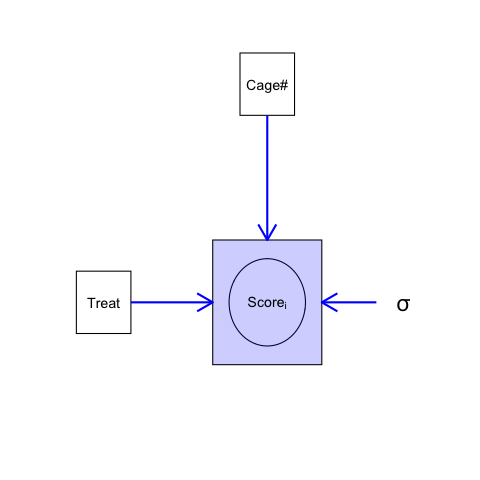
\includegraphics[width=6.67in]{../images/Lecture3_gm_vaccine} \end{center}

\end{block}

\end{frame}

\begin{frame}{Example 2: Drought resistance in GM tomato plants}
\protect\hypertarget{example-2-drought-resistance-in-gm-tomato-plants}{}

\begin{itemize}
\item
  Genotypes: WT or mutant
\item
  watering conditions: normal or drought
\item
  Outcome: leaf temperature at 7 days post-treatment
\item
  Potential \emph{factors} influencing score: genotype (2) and treatment
  (2)
\item
  Estimate \emph{treatment effect} within each genotype
\item
  Do treatment effects differ by genotype?
\end{itemize}

\end{frame}

\begin{frame}{Example 2: Drought resistance in GM tomato plants}
\protect\hypertarget{example-2-drought-resistance-in-gm-tomato-plants-1}{}

\begin{block}{Proposed data generating process}

\begin{center}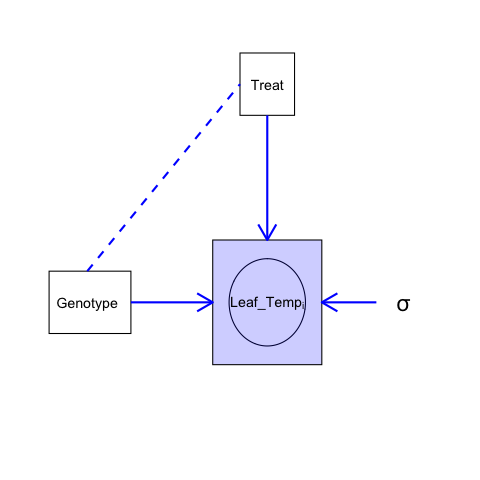
\includegraphics[width=6.67in]{../images/Lecture3_drought} \end{center}

\end{block}

\end{frame}

\begin{frame}{Example 3: Diet and obesity}
\protect\hypertarget{example-3-diet-and-obesity}{}

\begin{block}{Are NODk mice more susceptible to obesity with a high fat
diet?}

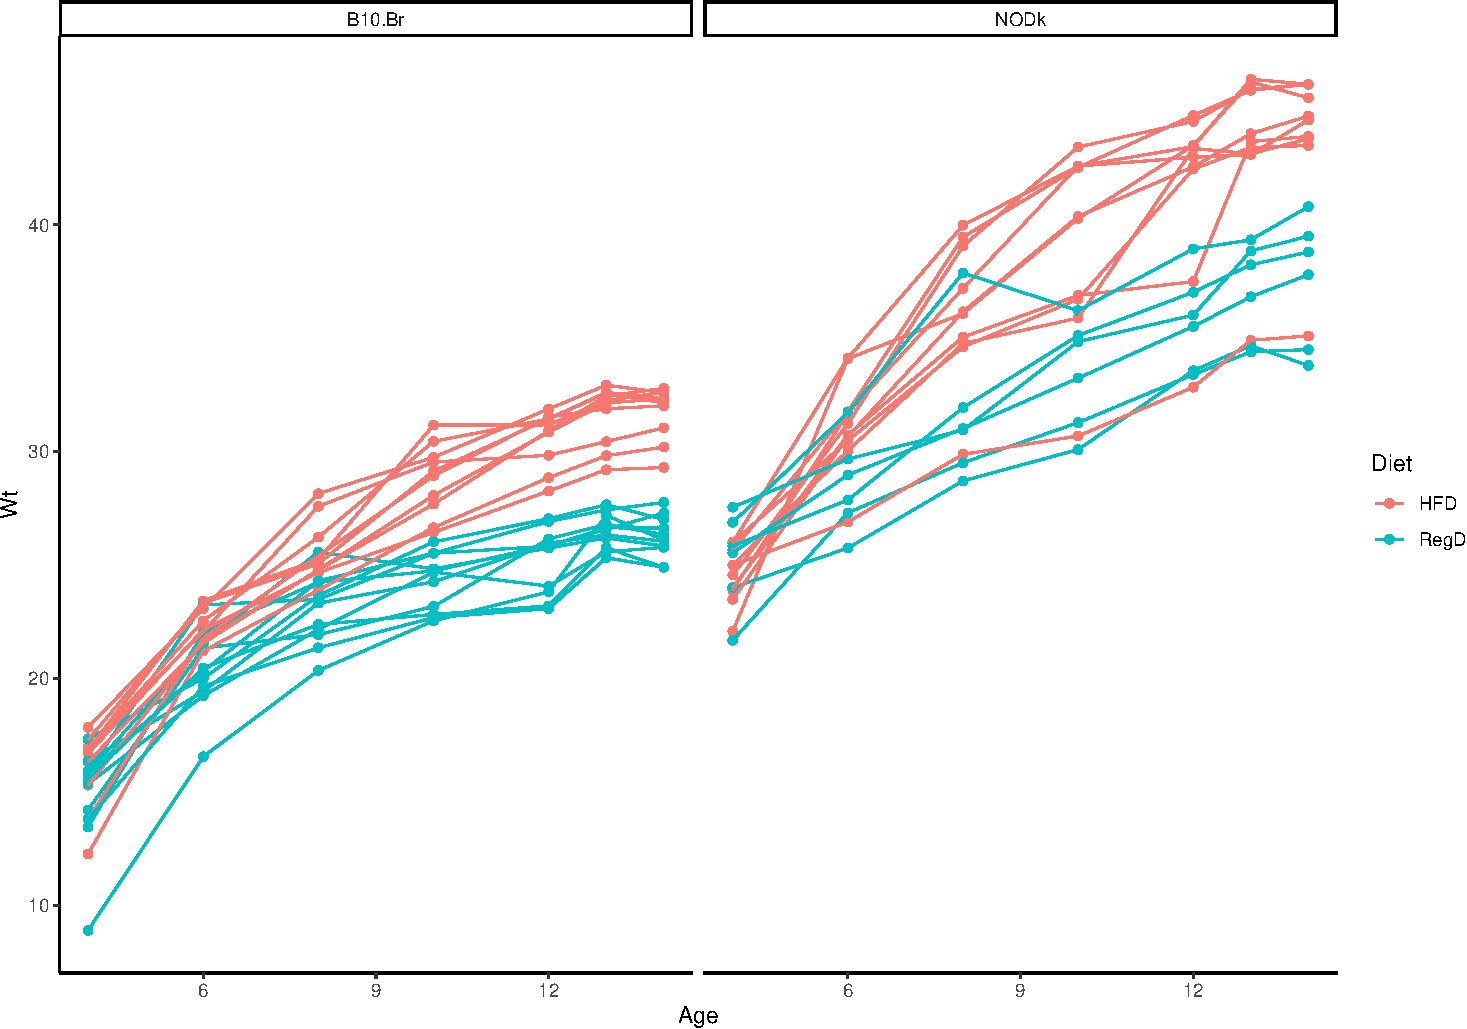
\includegraphics{Lecture-3_files/figure-beamer/unnamed-chunk-3-1.pdf}

\end{block}

\end{frame}

\begin{frame}{Example 3: Diet and obesity}
\protect\hypertarget{example-3-diet-and-obesity-1}{}

\begin{block}{Are NODk mice more susceptible to obesity with a high fat
diet?}

\begin{itemize}
\tightlist
\item
  Genotypes: WT or NODk
\item
  Diet: normal or high fat
\item
  Age: measured over time
\end{itemize}

\begin{block}{Does diet impact \emph{growth}? Does diet have stronger
impact on NODk mice?}

\end{block}

\end{block}

\end{frame}

\begin{frame}{Example 3: Diet and obesity}
\protect\hypertarget{example-3-diet-and-obesity-2}{}

\begin{center}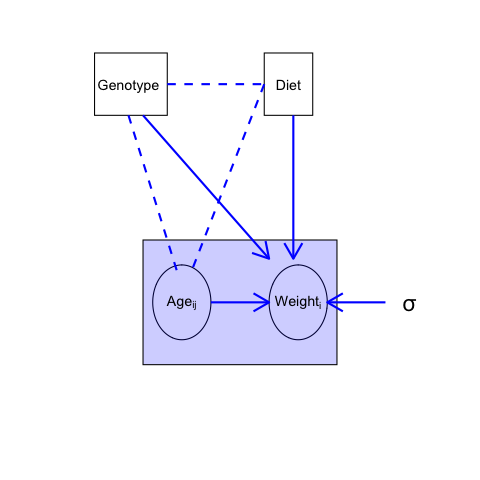
\includegraphics[width=6.67in]{../images/Lecture3_diet} \end{center}

\end{frame}

\begin{frame}{Summary}
\protect\hypertarget{summary}{}

\begin{itemize}
\item
  Statistical models: conceptualisation of experiment
\item
\end{itemize}

\begin{block}{In the next workshop, we'll fit models to data using R}

\end{block}

\end{frame}

\end{document}
